\chapter{Los glóbulos rojos en el cuerpo humano}\label{chap:RBC}
\section{Introducción}\label{sec:RBC:intro}
Este capítulo estará basado en los textos de Schippel \cite{schippel2023dynamics}, Hall \cite{hall2021guyton} y Thiagarajan \cite{thiagarajan2021red}. Se evidenciarán las funciones y dinámicas de los glóbulos rojos en el cuerpo humano desde una perspectiva completamente médica.

La \textbf{hematología} es el estudio biológico de la sangre, de sus componentes y de los desordenes que puede tener que afecten directamente el cuerpo humano. El estudio de la sangre es muy importante para la medicina ya que es una de las sustancias más abundantes del cuerpo, abarcando cerca del 8\% de la masa corporal con una cantidad aproximada de 5 litros, y que tiene funciones muy importantes, como oxigenar todas las células para garantizar su correcto funcionamiento.

\section{Composición de glóbulos rojos}\label{sec:RBC:Composicion}
Los \textbf{glóbulos rojos} (RBC's, por sus siglas en inglés), o eritrocitos, son las células principales del sistema circulatorio en el cuerpo humano. Estos constituyen alrededor del 50\% de la sangre, concentrando entre cuatro y seis millones de células por milímetro cúbico de sangre y cerca de 25 trillones en total (\cite{enwiki:1217153817}), para hombres adultos su concentración está aproximadamente entre 21.75 y 28.25 trillones, y son fundamentales para la supervivencia humana, pues son los encargados de enviar oxigeno desde los pulmones hasta los diferentes órganos. Entre otras funciones, los eritrocitos transportan sustancias importantes para el cuerpo tales como aminoácidos y ácidos grasos. Adicionalmente, también son los encargados de enviar ciertas sustancias nocivas para el cuerpo a los órganos que las desechan, como lo puede ser el dióxido de carbono.

Los eritrocitos son células sin núcleo con forma de disco bicóncavo con un radio aproximado de 4 micrómetros que son muy flexibles dado que tienen un exceso de membrana celular. La principal sustancia que contienen los glóbulos rojos es la hemoglobina, una proteína hecha principalmente de hierro que es la encargada del transporte del oxígeno y del dióxido de carbono, esta proteína es la que le otorga el color rojizo a la sangre humana. De esta manera, el hierro es una sustancia fundamental para la producción de los glóbulos rojos, y un nivel bajo de este, así como de vitamina B y ácido fólico, puede perjudicar gravemente las dinámicas de los eritrocitos.

Entre otras sustancias que se encuentran dentro de los RBC's, hay enzimas en su citoplasma que permiten flexibilidad, transporte de iones, estabilización de la hemoglobina y logran impedir la oxidación de otras proteínas.

\section{Proceso de vida de los glóbulos rojos}\label{sec:RBC:vida}

El origen inicial de los RBC's se encuentra en las células madre hematopoyéticas ubicadas en la médula ósea mediante el proceso de la \textbf{eritropoyesis}. Al detectar cantidades bajas de oxígeno en la sangre, los riñones se encargan de sintetizar la \textbf{eritropoyetina} (EPO), la hormona clave en la producción de estas células que es medida en miliunidades por mililitro de sangre (mU/mL) y que tiene una concentración normal de entre 4 a 26 mU/ml (\cite{Cleveland}), para informarle al cerebro que debe producir más glóbulos rojos. 

Las células madre hematopoyéticas son las que producen todas las células necesarias para la sangre. Al recibir el comando de la eritropoyetina, estas inician un proceso de transformación, pasando a ser proeritroblastos que, al ser ya maduros, terminan dividiéndose y perdiendo el núcleo para convertirse finalmente en varios RBC's. Cada segundo, entre dos y tres millones de glóbulos rojos terminan su proceso de maduración y son colocados en el torrente sanguíneo para cumplir sus funciones.

\begin{figure}[H]
    \centering
    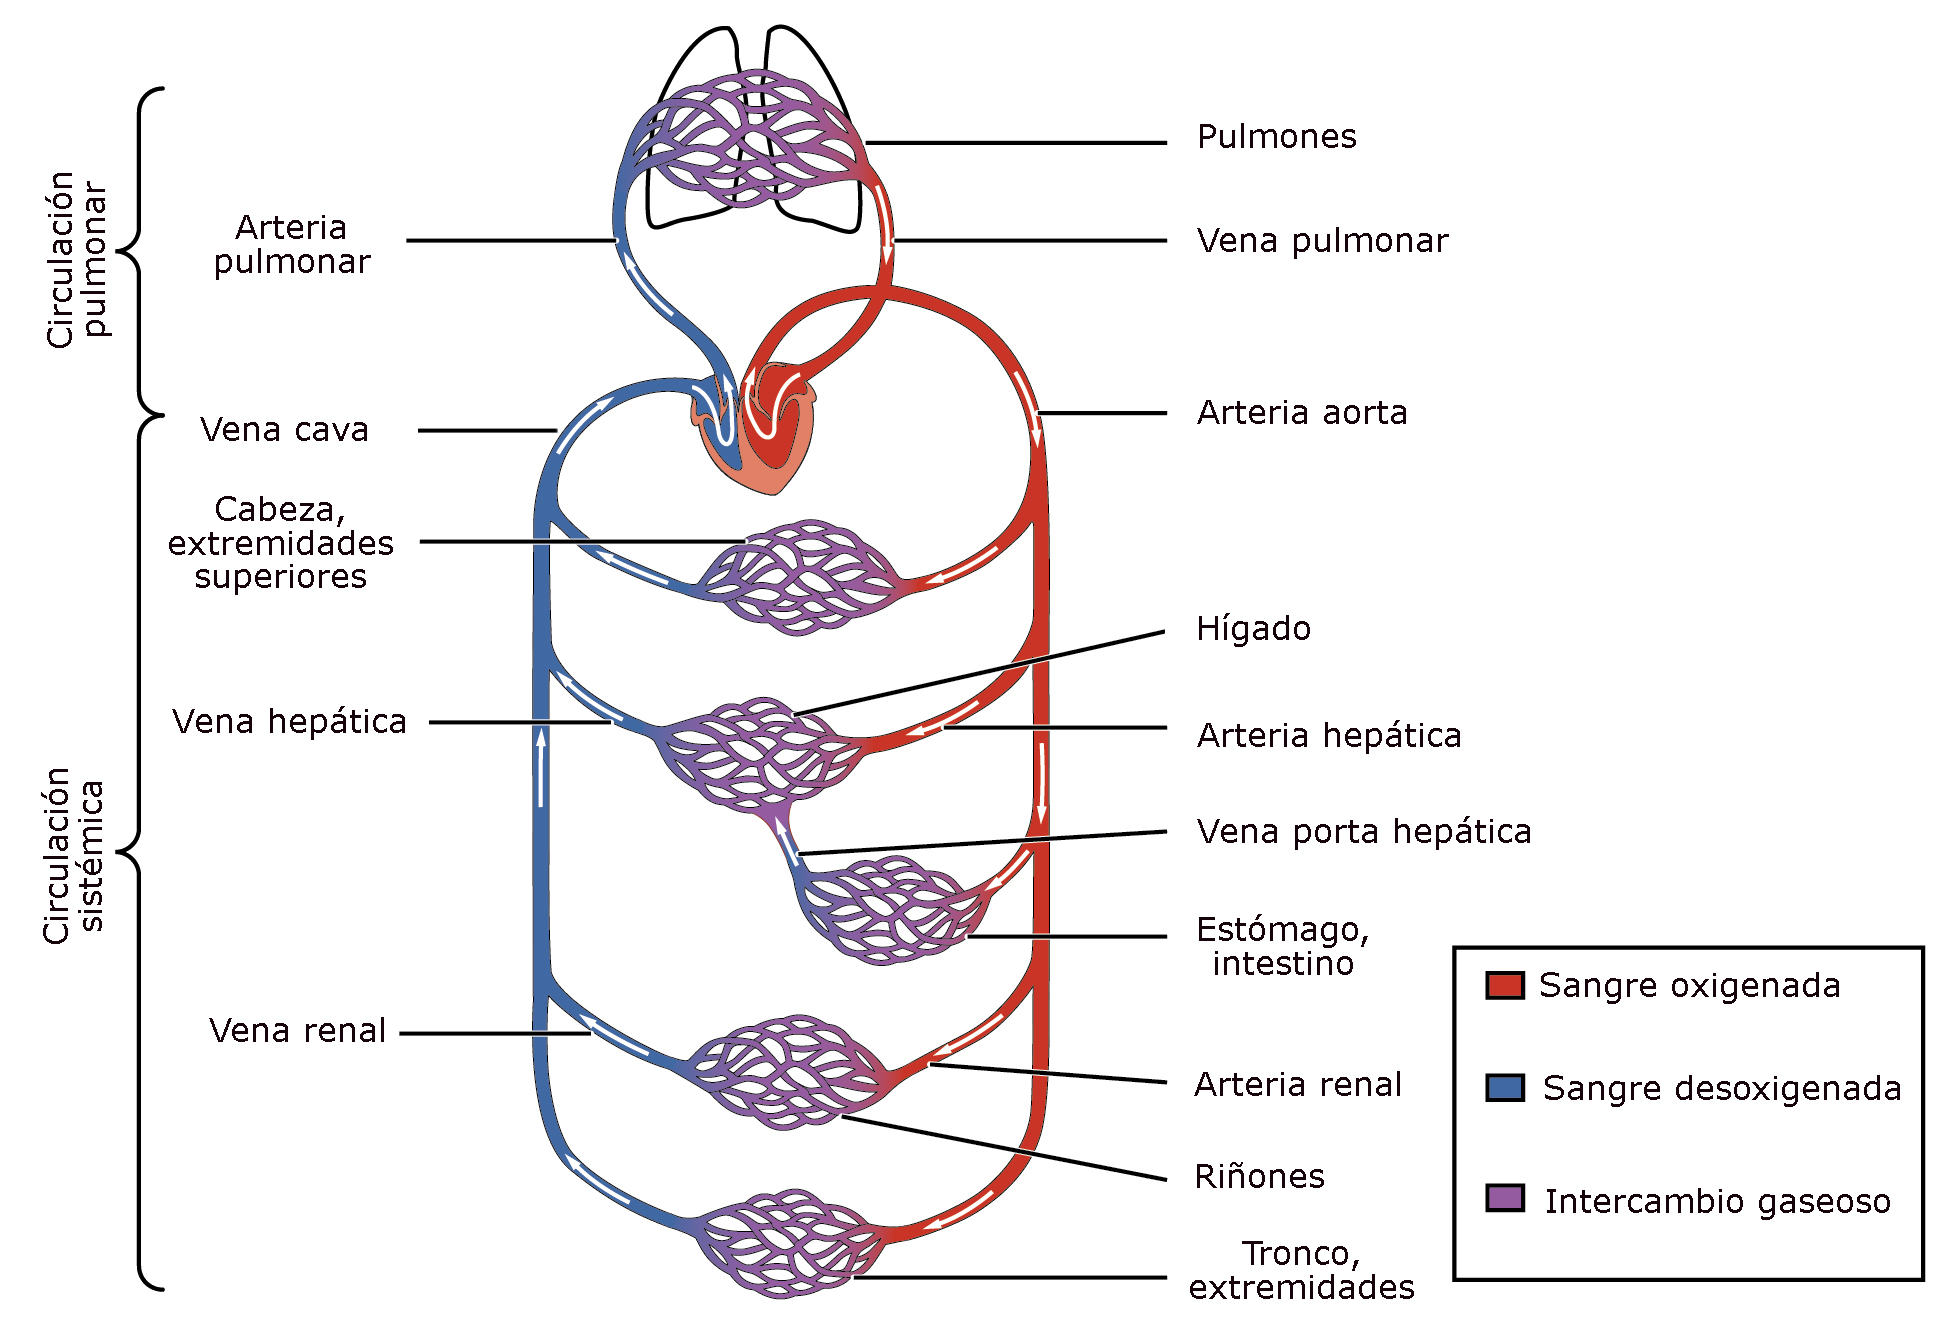
\includegraphics[scale=0.2]{figures/CicloSangre.jpg}
    \caption{El ciclo que cumple la sangre en el cuerpo humano. Imagen tomada de \cite{eswiki:159489943}.}
    \label{sec:RBC:fig:CicloSangre}
\end{figure}

Durante un periodo aproximado entre 90 y 120 días, unos tres o cuatro meses, los nuevos glóbulos rojos completan el ciclo cardíaco gracias a los bombeos del corazón, viajando de los pulmones, para recibir el oxigeno, hasta todos los órganos, para entregarles el oxigeno y recibir el dióxido de carbono, como se ilustra en la figura \ref{sec:RBC:fig:CicloSangre}. De esta manera, hacer una observación de la población de glóbulos rojos diaria es acertado, pues su ciclo de vida es medido en días.

Al cumplir su vida útil, la membrana de los glóbulos rojos está debilitada y su tamaño reducido, por lo que los eritrocitos pueden ser filtrados por el bazo y eliminados por el cuerpo. También es posible que, al ser más frágiles de lo normal, los RBC's exploten dentro del torrente sanguíneo, pero las células macrófagas de la sangre son capaces de digerirlos rápidamente. Para calcular la cantidad de eritrocitos que mueren al día, basta hacer el cálculo de 25 trillones de RBC's entre 120 días que es la vida promedio de estos, obteniendo un resultado aproximado de 208 billones de glóbulos rojos eliminados diariamente.

Contando con todo el ciclo expuesto, un diagrama compartimental, basado en aquel que se presenta en \cite{kirk1968mathematical}, que puede mostrar claramente el ciclo de vida de los glóbulos rojos es el siguiente:

\begin{figure}[H]
    \centering
    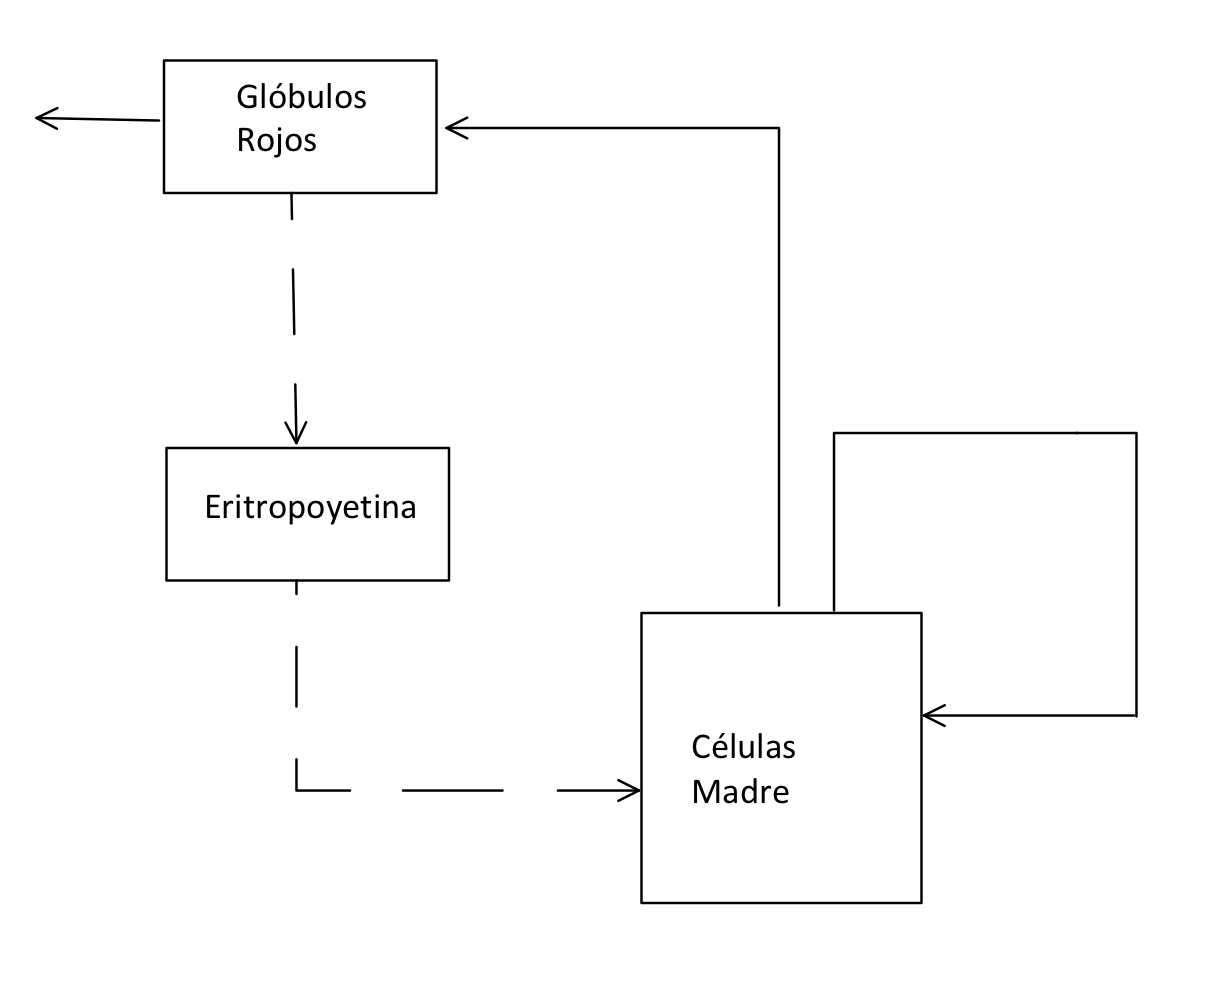
\includegraphics[scale=0.3]{figures/VidaRBC.jpeg}
    \caption{El proceso de producción y eliminación de glóbulos rojos.}
    \label{sec:RBC:fig:VidaRBC}
\end{figure}

En donde se desestima la transformación de células madre en otro tipo de células del cuerpo, fuera de la mitosis para autorreproducirse. La línea punteada implica que es bajo la acción de la eritropoyetina que las células madre reciben la señal de iniciar la eritropoyesis.

\section{Homeostasis}\label{sec:RBC:homeostasis}

Biológicamente, la \textbf{homeostasis} se define como la propiedad que tienen los organismos vivos de mantener un equilibrio estable al compensar pérdidas y ganancias. De esta manera, la hematología también es la encargada de estudiar la homeostasis de la sangre y de los glóbulos rojos en el cuerpo humano. Diferentes enfermedades o percances como la anemia, definida como el déficit de glóbulos rojos o de hemoglobina en la sangre, o las hemorragias deben de ser tenidas en cuenta para generar y simular un buen modelo matemático de las dinámicas de los glóbulos rojos en el cuerpo humano.

\section{Enfermedades y Complicaciones}\label{sec:RBC:enfermedades}

A la hora de construir un modelo matemático para las dinámicas de los glóbulos rojos, es importante considerar algunos factores externos que pueden perturbar la homeostasis como enfermedades o complicaciones médicas, pues no tener en cuenta estos factores hace que el modelo no sea realista. Para la presente investigación, se tendrán en cuenta la anemia y las hemorragias.

\subsection{Anemia}\label{subsec:RBC:enfermedades:anemia}
La \textbf{anemia}, siguiendo las definiciones de Portoles en \cite{portoles2021anemia} y de Heras en \cite{heras2023anemia}, es la deficiencia de hemoglobina en el cuerpo humano, para hombres esta se considera en valores menores a 13 gramos por decilitro de sangre y para mujeres en valores menores a 12 gramos por decilitro de sangre. Una de las variantes de la anemia es la \textbf{anemia renal}, se produce por deficiencia de eritropoyetina, de hierro o de otras sustancias importantes para la eritropoyesis que son sintetizadas por los riñones, esto quiere decir que la deficiencia de producción de glóbulos rojos es un factor importante a tener en cuenta para las causas de la anemia renal.

Los pacientes que sufren de anemia suelen presentar cansancio y falta de aire a causa de la deficiencia de oxígeno en el cuerpo, pues al no haber suficientes RBC's o hemoglobina, la cantidad de oxígeno transportada por medio de la sangre es mucho menor. Teniendo esto en cuenta, es importante resaltar que una anemia grave puede resultar mortal para el ser humano y que sumada a otras enfermedades, como la enfermedad renal crónica, puede resultar en problemas cardíacos, pues el corazón debe cambiar su funcionamiento para intentar mantener oxigenados los órganos.

Entre los posibles tratamientos para esta enfermedad está en el uso de agentes estimuladores de la eritropoyesis, como la eritropoyetina, el hierro y las transfusiones sanguíneas, ya que estos componentes son los que permiten el aumento de los glóbulos rojos en el cuerpo y, de esta manera, de la hemoglobina. Estos tratamientos, sin embargo, pueden tener efectos secundarios como complicaciones cardiovasculares o el aumento drástico del hierro en el cuerpo, que puede derivar en diabetes. La eritropoyetina se aplica mediante inyecciones subcutáneas (es decir en la piel) o directamente en una vena, para los pacientes con anemia renal se recomienda la aplicación de entre 50 y 100 unidades por kilogramo de masa corporal según la Mayo Clinic en \cite{MayoClinic}.

\subsection{Hemorragias}\label{subsec:RBC:enfermedades:hemorragias}
Una \textbf{hemorragia}, siguiendo las definiciones de Sánchez en \cite{Sanchez2000Hemorragias}, o sangrado, es la pérdida de sangre en el cuerpo, ya sea internamente o externamente. Las hemorragias tienen múltiples causas, como cortes o golpes, y son sumamente comunes entre los seres humanos. Las hemorragias leves, causadas por cortes superficiales o golpes suaves, no necesitan tratamiento, pues el mismo cuerpo es capaz de cerrar la herida para frenar el sangrado y recomponer los eritrocitos perdidos. Los sangrados fuertes, sin embargo, deben ser tratados con urgencia, pues la constante pérdida de grandes cantidades de sangre puede ocasionar graves complicaciones e, inclusive, la muerte. No hay cifras para diferenciar un sangrado leve de uno grave, pero es claro que si hay una gran o continua pérdida de sangre se debe actuar inmediatamente, pues puede ser causado por la ruptura de algún vaso sanguíneo importante o de algún órgano. Si un ser humano pierde cerca del $20\%$ de su cantidad habitual de sangre, esto puede causar un shock hipovolémico, es decir que los órganos empiezan a dejar de funcionar (\cite{PerdidaSangre}).

Los pacientes que han perdido mucha sangre pueden presentar, así como con los pacientes anémicos, un fuerte cansancio y dificultades para respirar, aunque también puede llegar a extremos como el mareo o los desmayos.

Para tratar una hemorragia grave se debe localizar la herida que la causa y tratarla inmediatamente, y para compensar la pérdida de sangre se debe hacer una transfusión sanguínea mediante vía intravenosa, que suele tardar entre 1 y 4 horas con bolsas de 250 mililitros de glóbulos rojos siguiendo las recomendaciones del centro de transfusión, tejidos y células de Granada en España en \cite{Granada}. 

Habiendo ya visto desde una perspectiva fisiológica las dinámicas de los glóbulos rojos en el cuerpo humano, se procederá a presentar y analizar un modelo matemático que intente imitar tales dinámicas.
